\subsection{Yukawa Coupling }\label{sec:CAFYukawa}
An analogous analysis can be carried out using the RG equations governing the Yukawa couplings, which depend on the gauge coupling at one loop. For simplicity, we will consider a single Yukawa coupling $\alpha_y$ with the following beta function
\begin{equation}
    \beta_y:=\mu \frac{\text{d}\alpha_y}{\text{d}\mu}=\alpha_y(c_1\alpha_g+c_2\alpha_y)\,,\label{eq:betay1loop}
\end{equation}
where $\alpha_y=\frac{y^2}{(4\pi)^2}$, and $c_1$, $c_2$ are constants, where in general $c_1<0$ and $c_2>0$. First, let us consider the case of a vanishing gauge coupling, i.e.\ $\alpha_g=0$. In this case, the solution is analogous to that of the pure gauge theory (see Eq.~\eqref{eq:solbetag1loop}), 
\begin{equation}
    \alpha_y=\frac{\alpha_{y_0}}{1-c_2 \alpha_{y_0} \ln \left(\frac{\mu}{\mu_0 }\right)}\,,
\end{equation}
with the crucial difference being that the constant $c_2$ is positive. Therefore, in the high energy limit $\mu\to\infty$ the denominator becomes negative, resulting in a non-physical branch. For $\mu<\mu_L$ with $\mu_L=\mu_0\exp(1/{c_2\alpha_{y_0}})$ the coupling is positive. Thus, the coupling flows to the Gaussian fixed point in the IR and flows towards a Landau pole in the UV. This establishes that the Yukawa coupling can never be asymptotically free in the absence of a gauge coupling. Thus, when the gauge coupling flows to zero in the UV, so must the Yukawa coupling as fast as $\alpha_g$ or faster, to ensure that the contribution of the gauge coupling to the Yukawa beta function (Eq.~\eqref{eq:betay1loop}) remains sizeable. 

Let us turn to the case of $\alpha_g\neq0$. We now have a system of two coupled differential equations. A solution can be found utilising the ratio method \cite{Pendleton:1980as} on the Yukawa (Eq.~\eqref{eq:betay1loop}) and gauge (Eq.~\eqref{eq:betag1loopcaf}) beta functions 
\begin{align}
    \frac{\beta_y}{\beta_g}=\frac{\text{d}\alpha_y}{\text{d}\alpha_g}&= \frac{\alpha_y(c_1 \alpha_g + c_2 \alpha_y)}{b_0 \alpha_g^2} = \frac{\alpha_y}{b_0 \alpha_g} \left( c_1 + c_2 \frac{\alpha_y}{\alpha_g} \right)\,.\label{eq:betayfrac}
\end{align}
The solutions to the differential equation depend on $b_0$ and $c_1$. 

\paragraph{Case 1 $b_0=c_1$:} In this case the solution is given by 
\begin{equation}
    \alpha_y=\frac{\alpha_{y_0}}{\alpha_{g_0}\left(1+\frac{c_2}{c_1}\frac{\alpha_{y_0}}{\alpha_{g_0}}\ln\alpha_{g_0}\right)-\frac{c_2}{c_1}\alpha_{y_0}\ln \alpha_g }\alpha_g\,,\label{eq:ysolb0c1}
\end{equation}
with the initial condition $\alpha_y(\alpha_{g_0})=\alpha_{y_{0}}$. As $\alpha_g\to0$ the denominator will be dominated by the second term  $(-\frac{c_2}{c_1}\alpha_{y_0}\ln \alpha_g) $, since the logarithm of the gauge coupling will go towards negative infinity. Because the constant in front will always be negative $\frac{c_2}{c_1}<0$, the $\alpha_y$ coupling will be negative. Thus, we have no CAF solution in this case, since the Yukawa coupling follows a non-physical branch as the gauge coupling goes to zero, and we approach the UV. 

\paragraph{Case 2 $b_0\neq c_1$:} The solution changes to
\begin{equation}
    \alpha_y=\frac{\alpha_{y_0}}{ \alpha_g^{1-\frac{c_1}{b_0}}\alpha_{g_0}^{\frac{c_1}{b_0}}\left(1-\frac{c_2}{b_0-c_1}\frac{\alpha_{y_0}}{\alpha_{g_0}}\right)+\frac{c_2}{b_0-c_1}\alpha_{y_0} }\alpha_g\,.\label{eq:sol2g}
\end{equation}
The equation can be divided into two parts, one which will be dependent on $\alpha^{\frac{c_1}{b_0}}_g$ and one on $\alpha_g$. If $\frac{c_1}{b_0}>1$, the first term will dominate and for $\frac{c_1}{b_0}<1$ the second term will dominate. The case of $\frac{c_1}{b_0}=1$ has already been ruled out by the analysis of Eq.~\eqref{eq:ysolb0c1}. In the case of $\frac{c_1}{b_0}<1$, the coupling will go as 
\begin{equation}
    \alpha_y\sim\frac{b_0-c_1}{c_2}\alpha_g\,,\quad\quad 0>{c_1}>b_0\,,
\end{equation}
which is always negative, since $b_0-c_1<0$. Therefore, this scenario does not yield an asymptotically free Yukawa coupling. 

The final possibility is the regime where $\frac{c_1}{b_0}>1$. Here, the coupling behaves as
\begin{equation}
    \alpha_y\sim\frac{\alpha_{y_0}}{ \alpha_{g_0}^{\frac{c_1}{b_0}}\left(1-\frac{c_2}{b_0-c_1}\frac{\alpha_{y_0}}{\alpha_{g_0}}\right)}\alpha_g^{\frac{c_1}{b_0}}\,,\quad\quad \frac{\alpha_{g_0}}{\alpha_{y_0}}>\frac{c_2}{b_0-c_1}\,,\quad\quad c_1<b_0<0\,.\label{eq:Yukawacondoff}
\end{equation}
To ensure that the coupling will be positive, we need to constrain the values of the couplings at the RG reference scale: $\frac{c_2}{b_0-c_1}\frac{\alpha_{y_0}}{\alpha_{g_0}}<1$. In the UV, where $\alpha_g\to 0$, the Yukawa coupling will also be asymptotically free, and because $\frac{c_1}{b_0}>1$, the Yukawa coupling will go faster to zero than the gauge coupling at high energies. 

Another possibility is that the values of the couplings at the arbitrary energy level are fine-tuned $\frac{\alpha_{g_0}}{\alpha_{y_0}}=\frac{c_2}{b_0-c_1}$. In this case, the first term in the denominator in Eq.~\eqref{eq:sol2g} vanishes, and the previously dominated term is now the only one left:
\begin{equation}
    \alpha_y=\frac{b_0-c_1}{ c_2 }\alpha_g\,,\quad\quad \frac{\alpha_{g_0}}{\alpha_{y_0}}=\frac{c_2}{b_0-c_1}\,,\quad\quad b_0-c_1>0\,.\label{eq:ygfixed}
\end{equation}
This case is known as fixed flow \cite{Giudice:2014tma}. Along this trajectory, the Yukawa coupling vanishes with the same rate as the gauge coupling, i.e.\ the ratio $\alpha_y/\alpha_g$ flows to a constant. 

Thus, there are two ways to obtain a CAF regime for a system with a single gauge and Yukawa coupling: the couplings must follow either a fixed-flow trajectory (Eq.~\eqref{eq:ygfixed}) or an off-fixed-flow trajectory (Eq.~\eqref{eq:Yukawacondoff}). This distinction is illustrated by the RG flow plot in Figure~\ref{fig:gYCAFplot}. The values of the coefficients $b_0$ and $c_1$ are chosen such that they satisfy the CAF conditions (see Eq.~\ref{eq:Yukawacondoff}). The couplings exhibit fixed-flow behaviour only along the green trajectory. In this scenario, the values of the gauge and Yukawa couplings at the reference RG scale are more tightly constrained than in the off-fixed-flow regime, which corresponds to the region below the green line. Finally, trajectories above the green line do not exhibit CAF. This demonstrates the requirements on $\alpha_{g_0}$ as well as $\alpha_{y_0}$ to realise a CAF region, in addition to the constraints on the coefficients of the beta function (see Eq.~\eqref{eq:ygfixed}). 

\begin{figure}[h!]
    \centering
    \begin{subfigure}[b]{0.48\textwidth}
        \centering
        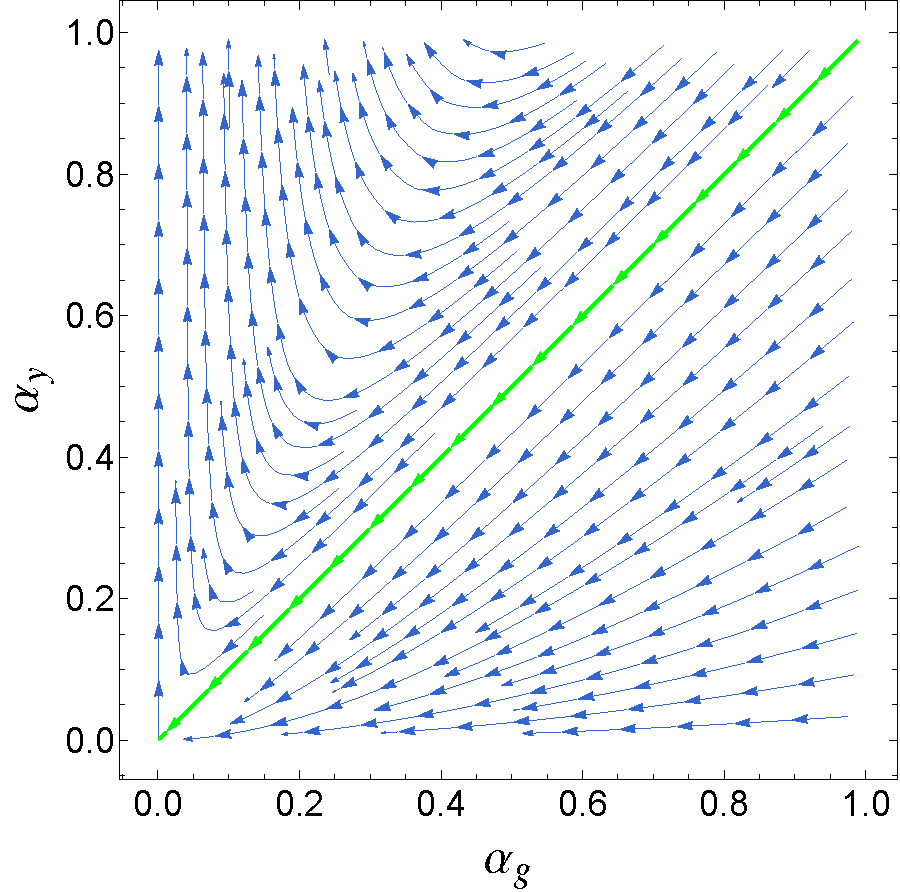
\includegraphics[width=\textwidth]{Figures/Flowplottest2.pdf}
        \caption{$(\alpha_g,\alpha_y)$} 
        \label{fig:gYCAFplot}
    \end{subfigure}%
    \hfill
    \begin{subfigure}[b]{0.48\textwidth}
        \centering
        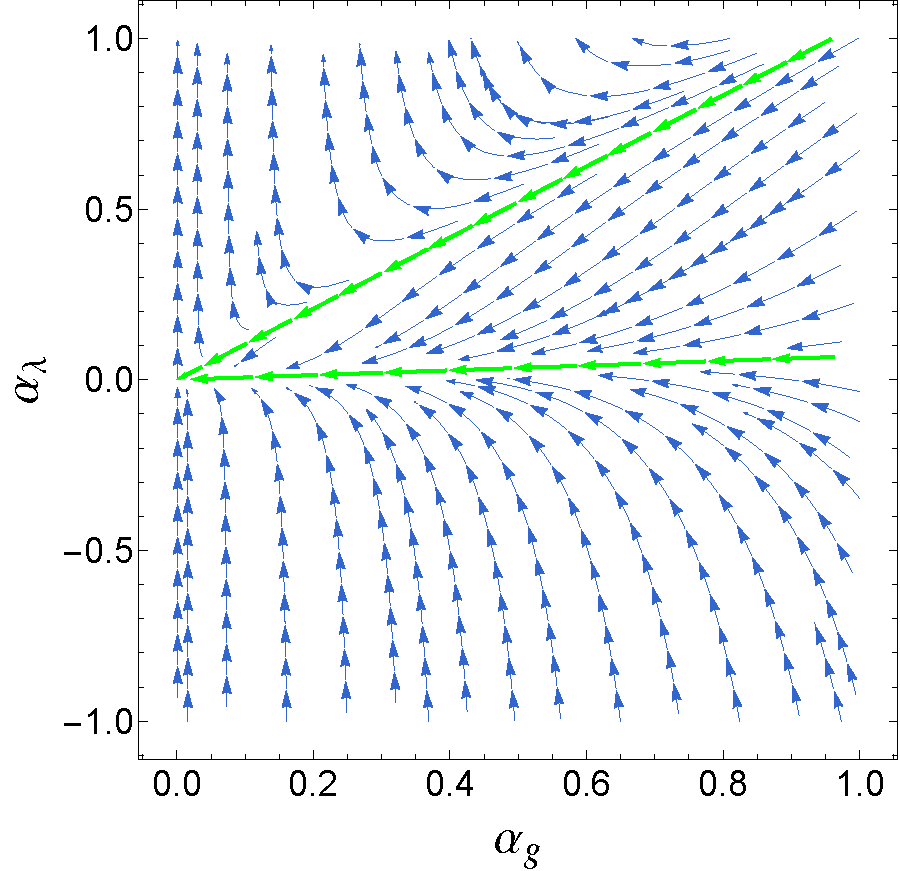
\includegraphics[width=\textwidth]{Figures/Scalarflow.pdf}
        \caption{$(\alpha_g,\alpha_\lambda)$}
        \label{fig:glamCAFplot}
    \end{subfigure}
    \caption{The RG flow of a CAF solution for all three couplings when the Yukawa coupling is off-fixed flow, thus upholding Eq.~\eqref{eq:CAF}. Panel (A) is in the $(\alpha_g,\alpha_y)$ parameter space and panel (B) is in the $(\alpha_g,\alpha_\lambda)$ parameter space. The green flow lines illustrate the fixed-flow of the couplings in the respective coupling space. All arrows point towards the UV and the values used were $b_0 = -2.0$, $c_1 = -4.0$, $c_2 = 0.9$, $d_1 = 7.0$, $d_2 = -12.0$, $d_3 = 1.0$, $d_4 = 1.0$, and $d_5 = -0.1$}
\label{fig:flowplottheory}
\end{figure}